\documentclass[a4paper,12pt]{article}
\usepackage[utf8]{inputenc}
\usepackage{listings}
\usepackage{amsmath, amssymb}
\usepackage{geometry}
\usepackage{booktabs}
\usepackage{graphicx}
\usepackage{tikz}
\usepackage{forest}
\usetikzlibrary{arrows.meta}
\usepackage{float}
\usepackage{tabularx}



\geometry{left=2.5cm, right=2.5cm, top=2.5cm, bottom=2.5cm}
\usepackage{fancyhdr}
\pagestyle{fancy}
\fancyhf{}
\lhead{Lösung zur Algorithmusanalyse}
\cfoot{\thepage}

\begin{document}
	
	\title{\textbf{Musterlösungen}}
	\date{\today}
	\maketitle
	
	\section*{Lösung zu Aufgabe 1: Analyse eines Algorithmus}
	\subsection*{Gegebener Java-Code}

\begin{verbatim}
	public class Algorithmus {
		public static int berechne(int n) {
			if (n <= 1) {
				return n;
			}
			return berechne(n - 1) + berechne(n - 2);
		}
		
		public static void main(String[] args) {
			int n = 5;
			System.out.println("Ergebnis: " + berechne(n));
		}
	}
\end{verbatim}
		
		\subsection*{1. Funktionsweise und mathematische Bedeutung}
		
		Der Algorithmus berechnet die $n$-te Zahl der Fibonacci-Folge. Diese ist rekursiv definiert durch:
		\[
		F(0) = 0,\quad F(1) = 1,\quad F(n) = F(n - 1) + F(n - 2)
		\]
		
		Die Methode \texttt{berechne(n)} ist eine direkte rekursive Umsetzung dieser Definition.
		
		\subsection*{2. Art der Implementierung}
		
		Es handelt sich um eine \textbf{rekursive Implementierung}. Vorteilhaft ist, dass sie sehr elegant ist und der mathematischen Definition entspricht. Sie ist jedoch ineffizient für große $n$, da viele Zwischenwerte mehrfach berechnet werden.
		
		\subsection*{3. Beispiel: Aufruf \texttt{berechne(5)}}
		
		Die rekursive Struktur lässt sich als Baum darstellen:

\begin{figure}[H]
	\centering
	\resizebox{\textwidth}{!}{
	\begin{forest}
		for tree={
			draw,
			rounded corners,
			align=center,
			edge={->},
			parent anchor=south,
			child anchor=north,
			grow'=south,
			l sep=12pt,
			s sep=8pt,
		}
		[berechne(5)
		[berechne(4)
		[berechne(3)
		[berechne(2)
		[berechne(1)\\1]
		[berechne(0)\\0]
		]
		[berechne(1)\\1]
		]
		[berechne(2)
		[berechne(1)\\1]
		[berechne(0)\\0]
		]
		]
		[berechne(3)
		[berechne(2)
		[berechne(1)\\1]
		[berechne(0)\\0]
		]
		[berechne(1)\\1]
		]
		]
	\end{forest}
}
	\caption{Rekursionsbaum für \texttt{berechne(5)}}
\end{figure}

		
		Am Ende ergibt sich:
		\[
		\texttt{berechne(5)} = \texttt{berechne(4)} + \texttt{berechne(3)} = 3 + 2 = 5
		\]
		
		\subsection*{4. Anzahl der Aufrufe für \texttt{berechne(5)}}
		
		Durch Zählen aller Knoten im Baum ergibt sich:
		\[
		\texttt{berechne(5)} \Rightarrow 15~\text{rekursive Aufrufe}
		\]
		
		\subsection*{5. Zeitkomplexität}
		
		Die Zeitkomplexität dieser rekursiven Lösung ist exponentiell:
		\[
		T(n) = T(n-1) + T(n-2) + \mathcal{O}(1) \Rightarrow \mathcal{O}(2^n)
		\]
		
		Grund: Jeder Aufruf erzeugt zwei weitere.
		
		\subsection*{6. Vergleich mit iterativer Lösung}
		
		Eine iterative Lösung speichert Zwischenwerte und vermeidet doppelte Berechnungen:
		
		\begin{lstlisting}[language=Java, caption=Iterative Berechnung]
			public static int fibonacciIterativ(int n) {
				if (n <= 1) return n;
				int a = 0, b = 1;
				for (int i = 2; i <= n; i++) {
					int temp = a + b;
					a = b;
					b = temp;
				}
				return b;
			}
		\end{lstlisting}
		
		\textbf{Vorteil:} Nur \(\mathcal{O}(n)\) Zeit und konstanter Speicherverbrauch.
		
		\subsection*{7. Optimierungsmöglichkeiten}
		
		\begin{itemize}
			\item \textbf{Memoization (Top-Down)}: Zwischenergebnisse werden gespeichert → \(\mathcal{O}(n)\) Zeit, rekursiv.
			\item \textbf{Bottom-Up (Iteration)}: Noch effizienter und speichersparend → \(\mathcal{O}(n)\) Zeit.
			\item \textbf{Dynamische Programmierung}: Allgemeiner Ansatz bei rekursiven Problemen mit überlappenden Teilproblemen.
		\end{itemize}
		
		\subsection*{8. Zusammenfassung}
		
		\begin{center}
			\begin{tabular}{|l|c|c|p{5cm}|}
				\hline
				\textbf{Variante} & \textbf{Zeit} & \textbf{Speicher} & \textbf{Bemerkung} \\
				\hline
				Rekursiv (naiv) & $\mathcal{O}(2^n)$ & Hoch (Call Stack) & Einfach, aber ineffizient \\
				\hline
				Iterativ & $\mathcal{O}(n)$ & Gering & Schnell, optimal für große $n$ \\
				\hline
				Rekursiv + Memo & $\mathcal{O}(n)$ & Mittel & Elegant und effizient \\
				\hline
			\end{tabular}
		\end{center}
		
		\section*{Aufgabe 2: Datenmodellierung und Normalisierung}
		
		Eine Schule speichert die Noten der Schüler in einer relationalen Datenbank. Die ursprüngliche Tabellenstruktur ist wie folgt:
		
		\begin{table}[h]
			\centering
			\caption{Ursprüngliche nicht normalisierte Tabelle}
			\begin{tabular}{|c|c|c|c|c|c|}
				\hline
				\textbf{SchülerID} & \textbf{Name} & \textbf{Klasse} & \textbf{Fach} & \textbf{Lehrer} & \textbf{Note} \\
				\hline
				101 & Max Meier & 10A & Mathematik & Herr Schmidt & 2 \\
				102 & Lisa Becker & 10A & Deutsch & Frau Müller & 1 \\
				101 & Max Meier & 10A & Deutsch & Frau Müller & 3 \\
				103 & Anna Keller & 10B & Englisch & Herr Weber & 2 \\
				102 & Lisa Becker & 10A & Mathematik & Herr Schmidt & 2 \\
				\hline
			\end{tabular}
		\end{table}
		
		\subsection*{1. Redundanzen in der Tabelle}
		
		\begin{itemize}
			\item Der Schülername 'Max Meier' taucht mehrfach auf.
			\item Die Klasse '10A' wird mehrfach gespeichert.
			\item Lehrer wie 'Herr Schmidt' erscheinen mehrfach mit identischem Fach.
			\item Fach-Lehrer-Zuordnungen sind redundant.
		\end{itemize}
		
		Dies führt zu höherem Speicherbedarf und potenzieller Fehleranfälligkeit (z.B. Tippfehler).
		
		\subsection*{2. Normalisierung bis zur 3. Normalform (3NF)}
		
		\textbf{1NF:} Bereits erfüllt, da alle Werte atomar sind.\\
		\textbf{2NF:} Es gibt partielle Abhängigkeiten (z.B. Name hängt nur von SchülerID ab). Daher Zerlegung in kleinere Tabellen:
		
		\subsubsection*{Tabelle: \texttt{Schueler}}
		
		\begin{tabular}{|c|l|c|}
			\hline
			\textbf{SchülerID} & \textbf{Name} & \textbf{Klasse} \\
			\hline
			101 & Max Meier & 10A \\
			102 & Lisa Becker & 10A \\
			103 & Anna Keller & 10B \\
			\hline
		\end{tabular}
		
		\vspace{1em}
		\subsubsection*{Tabelle: \texttt{Lehrer}}
		
		\begin{tabular}{|c|l|}
			\hline
			\textbf{LehrerID} & \textbf{Name} \\
			\hline
			L01 & Herr Schmidt \\
			L02 & Frau Müller \\
			L03 & Herr Weber \\
			\hline
		\end{tabular}
		
		\vspace{1em}
		\subsubsection*{Tabelle: \texttt{Fach}}
		
		\begin{tabular}{|c|l|c|}
			\hline
			\textbf{FachID} & \textbf{Fachname} & \textbf{LehrerID} \\
			\hline
			F01 & Mathematik & L01 \\
			F02 & Deutsch & L02 \\
			F03 & Englisch & L03 \\
			\hline
		\end{tabular}
		
		\vspace{1em}
		\subsubsection*{Tabelle: \texttt{Noten}}
		
		\begin{tabular}{|c|c|c|}
			\hline
			\textbf{SchülerID} & \textbf{FachID} & \textbf{Note} \\
			\hline
			101 & F01 & 2 \\
			102 & F02 & 1 \\
			101 & F02 & 3 \\
			103 & F03 & 2 \\
			102 & F01 & 2 \\
			\hline
		\end{tabular}
		\\
		\\ \textbf{3NF:} Erfüllt, da keine transitiven Abhängigkeiten bestehen.
		
		\subsection*{3. Vorteile der Normalisierung}
		
		\begin{itemize}
			\item \textbf{Weniger Redundanz:} z.B. Lehrername nur einmal gespeichert
			\item \textbf{Bessere Datenintegrität:} Konsistente und korrekte Daten
			\item \textbf{Pflegeleichter:} Änderungen müssen nur an einer Stelle erfolgen
			\item \textbf{Skalierbarkeit:} Neue Fächer, Lehrer oder Schüler lassen sich leicht ergänzen
			\item \textbf{Fehlervermeidung:} Reduzierung von Tippfehlern und Inkonsistenzen
		\end{itemize}
\newpage				
\section*{Aufgabe 3: Analyse einer formalen Grammatik}

Gegeben sei die Grammatik \( G \) mit:

\begin{itemize}
	\item \textbf{Nichtterminale:} \( \{S, X, Y\} \)
	\item \textbf{Terminale:} \( \{0, 1\} \)
	\item \textbf{Produktionsregeln:}
	\begin{align*}
		S &\rightarrow 0 X 1 \\
		X &\rightarrow 0 X 1 \mid 1 Y 0 \\
		Y &\rightarrow 1 Y 0 \mid \epsilon
	\end{align*}
	\item \textbf{Startsymbol:} \( S \)
\end{itemize}

\subsection*{Sprachanalyse}

Die Grammatik \( G \) beschreibt Wörter der Form:
\[
w = 0^n \, 1^m \, 1^k \, 0^m \, 1^n \quad \text{mit } n \geq 1,\, m \geq 0,\, k \geq 0
\]
Diese Struktur ergibt sich aus:
\begin{itemize}
	\item jeder Anwendung von \( X \rightarrow 0 X 1 \) erzeugt symmetrisch äußere 0–1-Paare (Zähler \( n \))
	\item der abschließenden Regel \( X \rightarrow 1 Y 0 \), die einmalig vorkommen muss
	\item beliebiger Anzahl von \( Y \rightarrow 1 Y 0 \), die zentrale Mitte bildet (Zähler \( m \))
	\item \( Y \rightarrow \epsilon \) schließt die Mitte ab
\end{itemize}

\subsection*{Überprüfung der Wörter}

\textbf{Wort 1:} \( \texttt{000111000111} \)

\begin{itemize}
	\item Länge: 12
	\item Struktur: \( 000 \, 111 \, 000 \, 111 \)
	\item Es liegt eine gespiegelte Struktur vor:
	\[ \texttt{000} \, \texttt{1\underline{11}0} \, \texttt{111} \]
	\item Zerlegung möglich in:
	\[
	S \Rightarrow 0\, X\, 1 \\
	X \Rightarrow 0\, X\, 1 \\
	X \Rightarrow 0\, X\, 1 \\
	X \Rightarrow 1\, Y\, 0 \\
	Y \Rightarrow 1\, Y\, 0 \\
	Y \Rightarrow \epsilon
	\]
	\item Daraus ergibt sich:
	\[
	0\,0\,0\,1\,1\,1\,0\,0\,0\,1\,1\,1 = \texttt{000111000111}
	\]
\end{itemize}

\textbf{Fazit:} Das Wort \texttt{000111000111} gehört zur Sprache \( L(G) \).

\vspace{1em}

\textbf{Wort 2:} \( \texttt{000100011000} \)

\begin{itemize}
	\item Länge: 12
	\item Struktur nicht symmetrisch: Mittelteil ist nicht durch \( Y \) erklärbar
	\item Keine passende Ableitung der Form \( 0^n\,1^m\,1^k\,0^m\,1^n \)
	\item Beispiel: die Mitte \texttt{100011} verletzt das symmetrische Muster
\end{itemize}

\textbf{Fazit:} Das Wort \texttt{000100011000} gehört \textbf{nicht} zur Sprache \( L(G) \).

\subsection*{Teilfragen zur Grammatik}

\begin{enumerate}
	\item \textbf{Ableitung von \texttt{101}:}  
	Es gilt:  
	\[
	S \Rightarrow 0 X 1 \quad X \Rightarrow 1 Y 0 \quad Y \Rightarrow \epsilon
	\]
	\[
	\Rightarrow 0 \, 1 \, 0 \, 1 \neq \texttt{101}
	\]
	\texttt{101} kann \textbf{nicht} abgeleitet werden, da jedes Wort mit \texttt{0} beginnt und mit \texttt{1} endet.  
	\textbf{Fazit:} \texttt{101} gehört \textbf{nicht} zur Sprache \( L(G) \).
	
	\item \textbf{Kann die Grammatik alle Binärzahlen erzeugen?}  
	Nein, es können nur Wörter mit einer ganz bestimmten symmetrischen Struktur abgeleitet werden.  
	Die Grammatik erzeugt genau die Sprache:
	\[
	L(G) = \left\{ 0^n \, 1^m \, 1^k \, 0^m \, 1^n \mid n \geq 1, m \geq 0, k \geq 0 \right\}
	\]
	\textbf{Anpassungsidee:} Um beliebige Binärzahlen zu erzeugen:
	\[
	S \rightarrow 0 S \mid 1 S \mid \epsilon
	\]
	
	\item \textbf{Erweiterung für nur Wörter mit gerader Länge:}  
	Idee: immer zwei Zeichen pro Ableitung erzeugen:
	\[
	S \rightarrow 00 S \mid 01 S \mid 10 S \mid 11 S \mid \epsilon
	\]
	Jede Ableitung erzeugt exakt zwei Zeichen → Nur Wörter mit gerader Länge werden erzeugt.
\end{enumerate}


	
	
	
	
	
\newpage	
	
	
	
	\section*{Kolloquium-Antworten}
	\subsubsection*{Algorithmen}
	
	1. Welche Eigenschaften muss ein Algorithmus haben?\\
	Ein Algorithmus ist eine eindeutige Handlungsvorschrift zur Lösung eines Problems. Er muss folgende Eigenschaften besitzen:
	\begin{enumerate}		
		\item[-] Finitheit (Endlichkeit): Der Algorithmus muss nach einer endlichen Anzahl von Schritten terminieren.
		\item[-] Eindeutigkeit (Determinismus): Jeder Schritt des Algorithmus muss klar definiert und eindeutig sein.
		\item[-] Ausführbarkeit: Jeder Schritt muss tatsächlich ausführbar sein (z.B. mit einem Computer).
		\item[-] Eingabe: Ein Algorithmus besitzt null oder mehr Eingabewerte, auf denen er operiert.
		\item[-] Ausgabe: Ein Algorithmus liefert mindestens eine Ausgabe, also ein Ergebnis.
		\item[-] Effektivität: Jeder Schritt muss in endlicher Zeit mit den gegebenen Ressourcen ausführbar sein.
	\end{enumerate}
	2. Warum ist die iterative Lösung oft effizienter als eine rekursive Lösung?\\
	\begin{enumerate}
		\item[-] Speicherverbrauch: Iterative Lösungen benötigen in der Regel weniger Speicher, da sie keine zusätzliche Speicherstruktur wie den Call-Stack (für Funktionsaufrufe) beanspruchen
		\item[-] Overhead: Jeder rekursive Funktionsaufruf erzeugt Overhead durch das Ablegen von Rücksprungadressen und lokalen Variablen im Stack.
		\begin{verbatim}
		def factorial(n):
		if n == 0:
		return 1
		return n * factorial(n - 1)
		\end{verbatim}
		
		\begin{verbatim}
		factorial(3)
		→ 3 * factorial(2)
		→ 3 * (2 * factorial(1))
		→ 3 * (2 * (1 * factorial(0)))
		→ 3 * (2 * (1 * 1))
		→ 6	
		\end{verbatim}
		Stack-Aufbau (von oben nach unten)
		\begin{verbatim}
			factorial(3)   → wartet auf Ergebnis von factorial(2)
			factorial(2)   → wartet auf Ergebnis von factorial(1)
			factorial(1)   → wartet auf Ergebnis von factorial(0)
			factorial(0)   → gibt 1 zurück (Basisfall)
		\end{verbatim}
		Rückweg / Stack wird abgearbeitet
		\begin{verbatim}
			factorial(0) → gibt 1 zurück
			factorial(1) → 1 * 1 = 1
			factorial(2) → 2 * 1 = 2
			factorial(3) → 3 * 2 = 6
		\end{verbatim}
		
		\item[-] Ausführungszeit: Iterationen sind oft schneller, da sie keine wiederholten Funktionsaufrufe verursachen.
		
		\item[-] Begrenzung: Rekursion kann z.B. aufgrund einer Sematikfehlers zum Stack Overflow führen, wenn zu viele Aufrufe ineinander verschachtelt werden.
		\begin{verbatim}
			def factorial(n):
			if n == 0:
			return 1
			return n * factorial(n + 1)
		\end{verbatim}
	\end{enumerate}
		3. In welchen Fällen könnte Rekursion einer Iteration vorzuziehen sein?
		\begin{enumerate}
		\item[-] Eleganz und Lesbarkeit: Bei Problemen mit natürlicher rekursiver Struktur (z.B. Divide-and-Conquer-Strategien bei Margesort oder Quicksort, Fakultät, Fobonacci) ist Rekursion oft intuitiver.
		\item[-] Konzeptualisierung und Umsetzung vereinfachen: Auch wenn sie ggf. ineffizienter ist.
		\end{enumerate}
		4. Was versteht man unter einem effizienten Algorithmus? Welche Maßstäbe werden zur Effizienzbewertung verwendet?\\ \\
		Ein effizienter Algorithmus liefert die korrekte Lösung in möglichst kurzer Zeit und mit minimalem Ressourcenverbrauch.\\
		Maßstäbe zur Effizienzbewertung:
		\begin{enumerate}
			\item[-] Zeitkomplexität: Wie verändert sich die Rechenzeit in Abhängigkeit von der Eingabegröße nn?
			\item[-] Platzkomplexität (Speicherverbrauch): Wie viel zusätzlicher Speicher wird benötigt?
			\item[-] Best-, Average- und Worst-Case-Verhalten
		\end{enumerate}
		\textbf{\underline{Ziel ist, möglichst geringe Wachstumsraten bei zunehmender Eingabegröße zu erreichen.}}
		\newpage
		5. Wie analysiert man die Zeitkomplexität eines Algorithmus?
		\begin{enumerate}
			\item[-] Zähle die Anzahl der elementaren Operationen (z.B. Vergleiche, Zuweisungen) als Funktion von $n$.
			\item[-] Identifiziere Schleifen, rekursive Aufrufe, bedingte Anweisungen.
			\begin{table}[h!]
				\centering
				\begin{tabular}{|l|l|}
					\hline
					\textbf{Konstrukt} & \textbf{Typischer Zeitaufwand} \\
					\hline
					Einfache Schleife über $n$ & $\mathcal{O}(n)$ \\
					Zwei verschachtelte Schleifen & $\mathcal{O}(n^2)$ \\
					Drei verschachtelte Schleifen & $\mathcal{O}(n^3)$ \\
					Rekursion mit einem Aufruf pro Ebene & $\mathcal{O}(n)$ \\
					Rekursion mit zwei rekursiven Aufrufen & $\mathcal{O}(2^n)$ \\
					Binäre Suche & $\mathcal{O}(\log n)$ \\
					Schleife halbiert sich pro Schritt ($i = i // 2$) & $\mathcal{O}(\log n)$ \\
					Konstante Operation (z.\,B. $x = a + b$) & $\mathcal{O}(1)$ \\
					\hline
				\end{tabular}
				\caption{Faustregeln zur Abschätzung der Zeitkomplexität}
			\end{table}
			\\Beispiel: Zwei verschachtelte Schleifen $O(n^2)$
			\begin{verbatim}
				for i in range(n):
				for j in range(n):
				print(i + j)
			\end{verbatim}
			
			Beispiel: Gesucht wird eine Zahl zwischen 1-1000 durch das Raten? $2^k > 1000$
			\begin{align*}
				\text{Produktregel:} \quad & \log_b(x \cdot y) = \log_b(x) + \log_b(y) \\
				\text{Quotientenregel:} \quad & \log_b\left(\frac{x}{y}\right) = \log_b(x) - \log_b(y) \\
				\text{Potenzregel:} \quad & \log_b(x^a) = a \cdot \log_b(x) \\
				\text{Wurzelregel:} \quad & \log_b\left(\sqrt[n]{x}\right) = \frac{1}{n} \cdot \log_b(x) \\
				\text{Basiswechsel:} \quad & \log_b(x) = \frac{\log_k(x)}{\log_k(b)}
			\end{align*}
			
			\begin{align*}
				\log_2(1000)=\frac{log_{10}(1000)}{log_{10}(2)}=\frac{3}{0,3010}=9,97
			\end{align*}
			
			\item[-] Nutze asymptotische Notation ($Big-O$, $Big-\Omega$, $Big-\Theta$) zur Klassifikation des Wachstums.
		\end{enumerate}
		6. Warum ist $O(n \ log(n))$ schneller als $O(n^2)$?
		\subsection*{Warum ist \( \mathcal{O}(n \log n) \) schneller als \( \mathcal{O}(n^2) \)?}
		
		Um das Wachstum zweier Funktionen zu vergleichen, bildet man ihr Verhältnis:
		
		\[
		\frac{n \log n}{n^2} = \frac{\log n}{n}
		\]
		
		Für \( n \to \infty \) gilt:
		
		\[
		\lim_{n \to \infty} \frac{\log n}{n} = 0
		\]
		
		Das bedeutet:
		\begin{itemize}
			\item \( n \log n \) wächst viel langsamer als \( n^2 \)
			\item Deshalb ist \( \mathcal{O}(n \log n) \subset \mathcal{O}(n^2) \)
		\end{itemize}
		
		\vspace{1em}
		
		\textbf{Beispielhafte Werte:}
		
		\begin{center}
			\begin{tabular}{@{}cccc@{}}
				\toprule
				\( n \) & \( \log_2(n) \) & \( n \log_2(n) \) & \( n^2 \) \\
				\midrule
				10 & \(\approx 3.3\) & \(\approx 33\) & 100 \\
				100 & \(\approx 6.6\) & \(\approx 660\) & 10\,000 \\
				1000 & \(\approx 10\) & \(\approx 10\,000\) & 1\,000\,000 \\
				\bottomrule
			\end{tabular}
		\end{center}
		
		\textbf{Fazit:}  
		Ein Algorithmus mit Laufzeit \( \mathcal{O}(n \log n) \) ist für große \( n \) deutlich effizienter als einer mit \( \mathcal{O}(n^2) \).\\
		\\7. Was ist der Unterschied zwischen exponentiellen $O(2^n)$ und polynomiellen $O(n^k)$ Algorithmen?\\
		
		\textbf{Polynomielle Laufzeit:} \( \mathcal{O}(n^k) \), wobei \( k \) eine feste Konstante ist.
		
		\begin{itemize}
			\item Die Anzahl der Schritte wächst gemäß eines Polynoms in \( n \)
			\item Beispiele: \( O(n) \), \( O(n^2) \), \( O(n^3) \)
			\item Auch für große Eingaben praktikabel
		\end{itemize}
		
		\vspace{0.5em}
		\textbf{Exponentielle Laufzeit:} \( \mathcal{O}(2^n) \), \( \mathcal{O}(3^n) \), \( \mathcal{O}(n!) \)
		
		\begin{itemize}
			\item Die Anzahl der Schritte verdoppelt oder vervielfacht sich mit jedem zusätzlichen Eingabeelement
			\item Wächst extrem schnell – unpraktisch für große \( n \)
			\item Beispiel: Brute-Force für das Rucksackproblem, naive Fibonacci-Berechnung
		\end{itemize}
		
		\vspace{1em}
		\textbf{Wachstumsvergleich:}
		
		\begin{center}
			\begin{tabular}{|c|c|c|c|}
				\hline
				\( n \) & \( n^2 \) & \( n^3 \) & \( 2^n \) \\
				\hline
				5      & 25        & 125       & 32 \\
				10     & 100       & 1000      & 1024 \\
				20     & 400       & 8000      & 1\,048\,576 \\
				50     & 2\,500    & 125\,000  & \(\sim 10^{15}\) \\
				100    & 10\,000   & 1\,000\,000 & \(\sim 10^{30}\) \\
				\hline
			\end{tabular}
		\end{center}
		
		\vspace{1em}
		\textbf{Fazit:} Polynomielle Algorithmen sind deutlich effizienter und für große Eingaben geeignet.\\
		Exponentielle Algorithmen explodieren im Aufwand und sind nur für kleine Eingaben sinnvoll.\\
		\\8. Wie kann man den Speicherverbrauch eines Algorithmus reduzieren?\\
		
		\begin{itemize}
			\item \textbf{In-Place-Operationen:} Verwende vorhandene Speicherplätze, anstatt neue Datenstrukturen anzulegen.
			\begin{itemize}
				\item Beispiel: \texttt{list.sort()} statt \texttt{sorted(list)}
			\end{itemize}
			
			\item \textbf{Vermeidung unnötiger Datenstrukturen:} Nutze nur das, was wirklich benötigt wird (z.\,B. kein $array$ wenn auch $strig$ geht).
			
			\item \textbf{Iteration statt Rekursion:} Rekursive Aufrufe verbrauchen Stack-Speicher.
			\begin{itemize}
				\item Beispiel: Iterative Fibonacci-Version spart Speicher gegenüber rekursiver.
			\end{itemize}
			
			\item \textbf{Nicht mehr benötigte Daten löschen:} Mit \texttt{del} oder durch Überschreiben Speicher freigeben. In Java über übernimmt diese Funktion der sog. Garbage Collectors (GC)
			
			\item \textbf{Effizientere Datenrepräsentation:} Nutze kompakte Datentypen. Z.B. $int$ statt $double$.
			
			\item \textbf{Teile-und-Herrsche optimieren:} Achte bei rekursiven Algorithmen darauf, keine überflüssigen Kopien zu erzeugen.
		\end{itemize}
		
		\vspace{1em}
		\textbf{Typische Speicherkomplexitäten:}
		
		\begin{center}
			\begin{tabular}{|l|c|}
				\hline
				\textbf{Struktur / Technik} & \textbf{Speicherbedarf} \\
				\hline
				einfache Schleife & \( O(1) \) \\
				Liste mit \( n \) Elementen & \( O(n) \) \\
				Rekursion (Call-Stack) & \( O(n) \) \\
				Memoisierung / DP-Tabellen & \( O(n) \) oder \( O(n^2) \) \\
				\hline
			\end{tabular}
		\end{center}
		
		\textbf{Fazit:}  
		Durch gezielte Optimierungen wie In-Place-Verarbeitung, Generatoren und iterative Verfahren kann der Speicherverbrauch erheblich reduziert werden.\\
		\newpage 9. Schreiben Sie einen Algorithmus in Pseudo-Code, der zwei Variablen ohne eine zusätzliche Variable tauscht.
		\begin{verbatim}
			Eingabe: a, b (zwei Zahlen)
			a := a + b
			b := a - b
			a := a - b
			Ausgabe: a, b (getauscht)
		\end{verbatim}
		Beispiel: $a=5$ und $b=9$
		\begin{verbatim}
			a = 5, b = 9
			
			1. a = a + b = 5 + 9 = 14
			2. b = a - b = 14 - 9 = 5
			3. a = a - b = 14 - 5 = 9
		\end{verbatim}
		10. Können Sie eine weitere Möglichkeit, denselben Algorithmus mit Hilfe von boolescher Algebra zu implementieren?\\
		\begin{verbatim}
			Eingabe: a, b (zwei Ganzzahlen)
			a := a XOR b
			b := a XOR b
			a := a XOR b
			Ausgabe: a, b (getauscht)
		\end{verbatim}
		Beispiel: $5_2 = 0101$  und $9_2 = 1001$
		\begin{verbatim}
			a = 5 (0101)
			b = 9 (1001)
			
			1. a = 0101 XOR 1001 = 1100 → 12
			2. b = 1100 XOR 1001 = 0101 → 5
			3. a = 1100 XOR 0101 = 1001 → 9
		\end{verbatim}
\subsubsection*{Datenbanken}		
		\begin{enumerate}
			\item Warum ist die Normalisierung wichtig für eine relationale Datenbank?
			\item Wie lauten die Definitionen von drei Normalformen?
			
			\textbf{1. Normalform (1NF):}
			
			Eine Relation befindet sich in der \textbf{1. Normalform}, wenn:
			\begin{itemize}
				\item alle Attributwerte atomar (unteilbar) sind
				\item keine Wiederholungsgruppen (z.\,B. mehrere Noten in einer Spalte) vorhanden sind
			\end{itemize}
			
			\textbf{Beispiel:}  
			Eine Spalte \texttt{Noten} mit dem Wert \texttt{2,3,1} wäre \textbf{nicht 1NF-konform}.  
			Korrekt wäre eine Zeile pro Note.
			
			\vspace{1em}
			
			\textbf{2. Normalform (2NF):}
			
			Eine Relation befindet sich in der \textbf{2. Normalform}, wenn:
			\begin{itemize}
				\item sie in 1NF ist
				\item jedes Nichtschlüsselattribut voll funktional abhängig vom gesamten Primärschlüssel ist
			\end{itemize}
			
			\textbf{Hinweis:} Gilt nur bei zusammengesetzten Primärschlüsseln.
			
			\textbf{Beispiel:}  
			Ist der Primärschlüssel \texttt{(SchuelerID, FachID)} und das Attribut \texttt{Name} hängt nur von \texttt{SchuelerID} ab, liegt eine \textbf{partielle Abhängigkeit} vor → Verstoß gegen 2NF.
			
			\vspace{1em}
			
			\textbf{3. Normalform (3NF):}
			
			Eine Relation befindet sich in der \textbf{3. Normalform}, wenn:
			\begin{itemize}
				\item sie in 2NF ist
				\item kein Nichtschlüsselattribut transitiv von einem Schlüssel abhängt
			\end{itemize}
			
			\textbf{Transitive Abhängigkeit:}  
			Wenn \( A \rightarrow B \) und \( B \rightarrow C \), dann ist \( C \) transitiv abhängig von \( A \)
			
			\textbf{Beispiel:}  
			Wenn \texttt{SchuelerID} → \texttt{Klasse} und \texttt{Klasse} → \texttt{Raum}, dann ist \texttt{Raum} transitiv abhängig von \texttt{SchuelerID} → Verstoß gegen 3NF.
			
			\vspace{1em}
			
			\textbf{Fazit:}  
			Die Normalformen dienen dazu, Redundanzen zu vermeiden, die Datenstruktur zu vereinfachen und Anomalien zu verhindern.
			
			\item Warum musste die ursprüngliche Tabelle normalisiert werden? Welche Probleme hätte es gegeben, wenn man sie in nicht normalisierter Form belassen hätte?
			\item Gibt es in der endgültigen normalisierten Form noch Redundanzen? Falls ja, sind diese gewollt?

			
			Ja, auch in der vollständig normalisierten Form (z.\,B. 3.\ Normalform oder Boyce-Codd-Normalform) können noch Redundanzen vorkommen. Diese sind jedoch in der Regel \textbf{gewollt und funktional notwendig}.
			
			\begin{itemize}
				\item In relationalen Datenbanken werden Beziehungen durch \textbf{Fremdschlüssel} dargestellt.
				\item Ein Fremdschlüssel (z.\,B. \texttt{SchuelerID}) kann in einer anderen Tabelle mehrfach vorkommen (z.\,B. in der Notentabelle).
				\item Diese Wiederholungen sind keine ungewollte Redundanz, sondern \textbf{essentiell}, um Relationen auszudrücken.
			\end{itemize}
			
			\subsubsection*{2. Kontrollierte Redundanz zur Performanceoptimierung}
			
			\begin{itemize}
				\item In manchen Fällen werden gezielt zusätzliche Redundanzen eingeführt, um die Performance zu verbessern.
				\item Dies geschieht bewusst im Rahmen einer \textbf{Denormalisierung}.
				\item Beispiel: Ein häufig verwendeter Wert wird zusätzlich in einer Tabelle gespeichert, um teure Joins zu vermeiden.
			\end{itemize}
			
			
			
			Auch wenn eine Datenbank korrekt bis zur 3.\ Normalform (3NF) normalisiert ist, kann es in bestimmten Situationen sinnvoll sein, gezielt \textbf{kontrollierte Redundanz} einzuführen – zum Beispiel zur Performanceverbesserung oder zur leichteren Berichtserstellung.
			
			\subsubsection*{Beispiel: Schulsystem}
			
			\textbf{Normalisierte Struktur:}
			
			\begin{itemize}
				\item \textbf{Schueler:}
				\begin{tabular}{|c|l|c|}
					\hline
					\textbf{SchuelerID} & \textbf{Name} & \textbf{Klasse} \\
					\hline
					101 & Max Meier & 10A \\
					\hline
				\end{tabular}
				
				\vspace{0.5em}
				\item \textbf{Lehrer:}
				\begin{tabular}{|c|l|}
					\hline
					\textbf{LehrerID} & \textbf{Name} \\
					\hline
					L01 & Herr Müller \\
					\hline
				\end{tabular}
				
				\vspace{0.5em}
				\item \textbf{Fach:}
				\begin{tabular}{|c|l|c|}
					\hline
					\textbf{FachID} & \textbf{Bezeichnung} & \textbf{LehrerID} \\
					\hline
					F01 & Mathematik & L01 \\
					\hline
				\end{tabular}
				
				\vspace{0.5em}
				\item \textbf{Noten:}
				\begin{tabular}{|c|c|c|}
					\hline
					\textbf{SchuelerID} & \textbf{FachID} & \textbf{Note} \\
					\hline
					101 & F01 & 2 \\
					\hline
				\end{tabular}
			\end{itemize}
			
			Diese Struktur ist vollständig normalisiert und vermeidet Redundanz.
			
			\subsubsection*{Kontrollierte Redundanz – gezielte Erweiterung}
			
			\textbf{Fall 1: Lehrername zusätzlich in der Noten-Tabelle speichern}
			
			\begin{tabular}{|c|c|c|l|}
				\hline
				\textbf{SchuelerID} & \textbf{FachID} & \textbf{Note} & \textbf{Lehrername} \\
				\hline
				101 & F01 & 2 & Herr Müller \\
				\hline
			\end{tabular}
			
			\textbf{Vorteil:} Lehrername ist direkt verfügbar, ohne dass ein JOIN mit der Lehrer- und Fach-Tabelle erforderlich ist.
			
			\vspace{1em}
			
			\textbf{Fall 2: Klasse direkt in der Noten-Tabelle speichern}
			
			\begin{tabular}{|c|c|c|l|}
				\hline
				\textbf{SchuelerID} & \textbf{FachID} & \textbf{Note} & \textbf{Klasse} \\
				\hline
				101 & F01 & 2 & 10A \\
				\hline
			\end{tabular}
			
			\textbf{Vorteil:} Schnellere Filterung nach Klassen, z.\,B. zur Anzeige aller Noten der Klasse 10A, ohne JOIN mit der Schueler-Tabelle.
			
			\subsubsection*{Fazit:}
			
			\begin{quote}
				Kontrollierte Redundanz bedeutet, dass Daten bewusst mehrfach gespeichert werden – z.\,B. zur Steigerung der Abfragegeschwindigkeit oder zur einfacheren Berichterstellung. Diese Redundanz ist zulässig, wenn sie gezielt eingesetzt und technisch (z.\,B. durch Trigger) gepflegt wird.\\
				In einer korrekt normalisierten Datenbankstruktur sind alle verbliebenen Redundanzen \textbf{gewollt und notwendig}. Sie unterstützen die Darstellung von Beziehungen (Fremdschlüssel) oder dienen der Effizienzsteigerung. \textbf{Unnötige Redundanzen}, die zu Anomalien führen können, werden durch die Normalisierung entfernt.
			\end{quote}
			
			
			\item Welche konkreten Redundanzen wurden durch die Normalisierung beseitigt?
			\item Welche Probleme können in einer nicht normalisierten Datenbank auftreten?\\
			
			In einer nicht normalisierten Datenbankstruktur treten verschiedene Probleme auf, die die Datenintegrität und Wartbarkeit beeinträchtigen. Im Folgenden sind die typischen Anomalien beschrieben:
			
			\subsubsection*{1. Redundanz (Datenwiederholung)}
			
			\begin{itemize}
				\item Gleiche Informationen werden mehrfach gespeichert, z.\,B. der Name eines Lehrers in jeder Zeile der Notentabelle.
				\item \textbf{Folgen:} unnötiger Speicherverbrauch, potenzielle Dateninkonsistenzen.
			\end{itemize}
			
			\vspace{0.5em}
			
			\subsubsection*{2. Änderungsanomalie (Update-Anomalie)}
			
			\begin{itemize}
				\item Eine Änderung muss an mehreren Stellen gleichzeitig durchgeführt werden.
				\item Beispiel: Der Name eines Lehrers ändert sich. Wird er nur an einer Stelle aktualisiert, entsteht Inkonsistenz.
			\end{itemize}
			
			\vspace{0.5em}
			
			\subsubsection*{3. Einfügeanomalie (Insert-Anomalie)}
			
			\begin{itemize}
				\item Neue Daten können nicht gespeichert werden, weil andere, abhängige Daten fehlen.
				\item Beispiel: Ein neues Fach soll erfasst werden, aber es gibt noch keinen Schüler mit einer Note darin → Einfügen nicht möglich.
			\end{itemize}
			
			\vspace{0.5em}
			
			\subsubsection*{4. Löschanomalie (Delete-Anomalie)}
			
			\begin{itemize}
				\item Beim Löschen eines Datensatzes gehen ungewollt auch andere, wichtige Informationen verloren.
				\item Beispiel: Wenn der letzte Schüler mit dem Fach Informatik gelöscht wird, verschwindet auch die Information, dass dieses Fach überhaupt existiert.
			\end{itemize}
			
			\vspace{0.5em}
			
			\subsubsection*{5. Fehlende Datenintegrität}
			
			\begin{itemize}
				\item Es gibt keine Zwangsregeln für gültige Datenbeziehungen.
				\item Beispiel: Ein Lehrername wird eingegeben, obwohl dieser Lehrer in keiner Lehrerliste erfasst ist.
			\end{itemize}
			
			\vspace{1em}
			
			\subsubsection*{Fazit}
			
			\begin{quote}
				In nicht normalisierten Datenbanken treten Redundanzen, Inkonsistenzen sowie Einfüge-, Änderungs- und Löschanomalien auf. Diese führen zu schlechter Wartbarkeit und einer hohen Fehleranfälligkeit. Die Normalisierung schafft klare Strukturen und verhindert solche Probleme.
			\end{quote}
			
			\item Gibt es Fälle, in denen man bewusst auf eine vollständige Normalisierung verzichtet? Warum?\\
			
			Ja, es gibt in der Praxis Fälle, in denen man bewusst auf eine vollständige Normalisierung verzichtet. Dieses Vorgehen wird als \textbf{Denormalisierung} bezeichnet.
			
			\subsubsection*{Gründe für gezielte Denormalisierung}
			
			\begin{enumerate}
				\item \textbf{Performance-Optimierung bei Abfragen}
				\begin{itemize}
					\item JOINs zwischen vielen Tabellen können bei großen Datenmengen die Abfrage verlangsamen.
					\item Durch kontrollierte Redundanz können Daten direkt in einer Tabelle bereitgestellt werden.
					\item Beispiel: Lehrername zusätzlich in der Noten-Tabelle speichern, um JOINs zu vermeiden.
				\end{itemize}
				
				\item \textbf{Einfachere Datenanalyse und Reporting}
				\begin{itemize}
					\item Analyse-Tools oder Excel arbeiten effizienter mit flachen Tabellen.
					\item Redundante Informationen vereinfachen Export und Auswertung.
				\end{itemize}
				
				\item \textbf{Bessere Lesbarkeit für Entwickler oder Benutzer}
				\begin{itemize}
					\item Eine leicht redundante Tabellenstruktur ist für bestimmte Zielgruppen einfacher zu verstehen.
					\item Besonders bei kleinen Projekten oder Einzeltabellen ist das akzeptabel.
				\end{itemize}
				
				\item \textbf{Weniger komplexe SQL-Abfragen}
				\begin{itemize}
					\item Statt komplexer Abfragen mit mehreren JOINs sind direkte Abfragen möglich.
					\item Dies reduziert Entwicklungsaufwand und Fehleranfälligkeit.
				\end{itemize}
				
				\item \textbf{Caching und Historisierung}
				\begin{itemize}
					\item In historischen Daten (z.\,B. Notenarchiv) soll der damalige Lehrername erhalten bleiben, auch wenn sich der Lehrer ändert.
					\item Deshalb wird der Name zusätzlich gespeichert.
				\end{itemize}
			\end{enumerate}
			
			\subsubsection*{Fazit}
			
			\begin{quote}
				In bestimmten Szenarien wird bewusst auf eine vollständige Normalisierung verzichtet, z.\,B. zur Performanceverbesserung, einfacheren Datenanalyse oder Datenarchivierung.  
				Diese \textbf{Denormalisierung} ist zulässig, wenn sie gezielt geplant und technisch kontrolliert erfolgt.
			\end{quote}
			
			\item Welche Normalform ist für den praktischen Einsatz am besten geeignet?\\
			
			In der Praxis hat sich die \textbf{3.\ Normalform (3NF)} als am besten geeignet erwiesen. Sie bietet einen guten Kompromiss zwischen \textbf{Redundanzfreiheit}, \textbf{Datenintegrität} und \textbf{praktischer Anwendbarkeit}.
			
			\vspace{1em}
			
			\subsubsection*{Vergleich der Normalformen}
			
			\begin{tabular}{|l|p{6cm}|p{5cm}|}
				\hline
				\textbf{Normalform} & \textbf{Eigenschaften} & \textbf{Praxis-Eignung} \\
				\hline
				1NF & Atomare Werte, keine Wiederholungsgruppen & Grundvoraussetzung jeder relationalen Datenbank \\
				\hline
				2NF & Keine partielle Abhängigkeit von zusammengesetzten Schlüsseln & Nur relevant bei zusammengesetzten Primärschlüsseln \\
				\hline
				\textbf{3NF} & Keine transitive Abhängigkeit von Nichtschlüsselattributen & \textbf{Sehr gut geeignet: Datenkonsistenz + überschaubare Struktur} \\
				\hline
				BCNF & Strengere Form der 3NF & In Spezialfällen notwendig, teilweise zu streng \\
				\hline
				4NF / 5NF & Behandeln mehrwertige und join-unabhängige Abhängigkeiten & Selten in Praxis, eher theoretisch relevant \\
				\hline
			\end{tabular}
			
			\vspace{1em}
			
			\subsubsection*{Vorteile der 3NF in der Praxis}
			
			\begin{itemize}
				\item Verhindert Redundanz und Anomalien (z.\,B. durch transitive Abhängigkeiten)
				\item Erzeugt übersichtliche Tabellenstrukturen
				\item Ist effizient genug für typische Anwendungen
				\item Wird von ORMs, Frameworks und SQL-Werkzeugen direkt unterstützt
			\end{itemize}
			
			\vspace{1em}
			
			\subsubsection*{Fazit}
			
			\begin{quote}
				Die \textbf{3.\ Normalform (3NF)} ist in der Praxis die am häufigsten verwendete Normalform. Sie bietet eine ausgewogene Balance zwischen theoretischer Datenbankstruktur und praktischer Effizienz. Höhere Normalformen (z.\,B. BCNF) werden nur bei speziellen Anforderungen benötigt.
			\end{quote}
			
			\item Gegeben sei eine relationale Datenbank mit folgenden Tabellen:
			
			\begin{itemize}
				\item \texttt{Schueler(SchuelerID, Name, Klasse)}
				\item \texttt{Lehrer(LehrerID, Name)}
				\item \texttt{Fach(FachID, Fachname, LehrerID)}
				\item \texttt{Noten(SchuelerID, FachID, Note)}
			\end{itemize}
			
			Formulieren Sie SQL-Abfragen für folgende Aufgaben:
			
			\begin{enumerate}
				\item Geben Sie den Namen aller Schüler aus, die in einem beliebigen Fach die Note \texttt{1} erhalten haben.
				
				\item Geben Sie zu jedem Noteneintrag den Namen des Schülers, den Fachnamen und den Namen des zugehörigen Lehrers aus.
				
				\item Ermitteln Sie für jede Klasse den Durchschnitt der Noten im Fach \texttt{Mathematik}.
			\end{enumerate}
			\subsection*{Lösungen: SQL-Abfragen zur Schüler–Lehrer–Noten–Datenbank}
			
			\textbf{Gegeben:}  
			Die folgenden Tabellen stehen zur Verfügung:
			
			\begin{itemize}
				\item \texttt{Schueler(SchuelerID, Name, Klasse)}
				\item \texttt{Lehrer(LehrerID, Name)}
				\item \texttt{Fach(FachID, Fachname, LehrerID)}
				\item \texttt{Noten(SchuelerID, FachID, Note)}
			\end{itemize}
			
			\subsubsection*{1. Schüler mit der Note 1}
			
			\begin{verbatim}
				SELECT s.Name
				FROM Schueler s
				JOIN Noten n ON s.SchuelerID = n.SchuelerID
				WHERE n.Note = 1;
			\end{verbatim}
			
			\textbf{Erläuterung:}  
			Verknüpfung von \texttt{Schueler} und \texttt{Noten}, Filterung nach Note = 1.
			
			\vspace{1em}
			
			\subsubsection*{2. Schülername, Fachname und Lehrername zu jeder Note}
			
			\begin{verbatim}
				SELECT s.Name AS Schuelername, f.Fachname, l.Name AS Lehrername
				FROM Noten n
				JOIN Schueler s ON n.SchuelerID = s.SchuelerID
				JOIN Fach f ON n.FachID = f.FachID
				JOIN Lehrer l ON f.LehrerID = l.LehrerID;
			\end{verbatim}
			
			\textbf{Erläuterung:}  
			Mehrfach-JOIN über alle vier Tabellen, um vollständige Informationen zu erhalten.
			
			\vspace{1em}
			
			\subsubsection*{3. Durchschnittsnote je Klasse im Fach Mathematik}
			
			\begin{verbatim}
				SELECT s.Klasse, AVG(n.Note) AS Durchschnitt
				FROM Noten n
				JOIN Schueler s ON n.SchuelerID = s.SchuelerID
				JOIN Fach f ON n.FachID = f.FachID
				WHERE f.Fachname = 'Mathematik'
				GROUP BY s.Klasse;
			\end{verbatim}
			
			\textbf{Erläuterung:}  
			Filterung nach \texttt{Mathematik}, Gruppierung nach Klasse, Durchschnittsberechnung mit \texttt{AVG()}.
			
			\subsection*{Einfache SQL-Abfragen (ohne JOINs)}
			
			\begin{enumerate}
				\item \textbf{Geben Sie alle Schüler aus der Klasse \texttt{10A} aus.}
				
				\begin{verbatim}
					SELECT * 
					FROM Schueler
					WHERE Klasse = '10A';
				\end{verbatim}
				
				\vspace{1em}
				
				\item \textbf{Geben Sie alle Fächer mit der FachID \texttt{F01} aus.}
				
				\begin{verbatim}
					SELECT * 
					FROM Fach
					WHERE FachID = 'F01';
				\end{verbatim}
				
				\vspace{1em}
				
				\item \textbf{Geben Sie alle Noten aus, die besser als \texttt{3} sind.}
				
				\begin{verbatim}
					SELECT * 
					FROM Noten
					WHERE Note < 3;
				\end{verbatim}
				
			\end{enumerate}
		\end{enumerate}
		\subsubsection*{Sprachen und Grammatiken}
		\begin{enumerate}
			\item Was versteht man unter einer formalen Sprache?\\
			Eine formale Sprache ist eine Menge von Wörtern über einem bestimmten Alphabet, die nach festen Regeln definiert sind.
			\item Was ist ein Alphabet?\\
			
			In der formalen Sprachtheorie bezeichnet ein \textbf{Alphabet} eine endliche, nichtleere Menge von Symbolen.
			
			\begin{itemize}
				\item Die Elemente eines Alphabets werden auch \textbf{Zeichen} oder \textbf{Symbole} genannt.
				\item Ein Alphabet wird üblicherweise mit dem griechischen Buchstaben \( \Sigma \) bezeichnet.
			\end{itemize}
			
			\textbf{Definition:}  
			Ein Alphabet ist eine endliche Menge:
			\[
			\Sigma = \{ a_1, a_2, \dotsc, a_n \}
			\]
			
			\textbf{Beispiele:}
			\begin{itemize}
				\item \( \Sigma_1 = \{0,1\} \) — binäres Alphabet
				\item \( \Sigma_2 = \{a, b, c\} \)
				\item \( \Sigma_3 = \{\texttt{A}, \texttt{C}, \texttt{G}, \texttt{T}\} \) — DNA-Zeichen
			\end{itemize}
			
			\textbf{Hinweis:}  
			Ein Alphabet enthält keine weiteren Informationen über die Bedeutung der Zeichen — es geht rein um die Menge der verwendbaren Symbole.
			
			\item Können Sie ein Beispiel für eine formale Sprache nennen?\\
			
			Eine \textbf{formale Sprache} ist eine Menge von Wörtern, die aus einem gegebenen Alphabet gebildet wurden und bestimmten Regeln folgen.
			
			\textbf{Beispiel:}  
			Gegeben sei das Alphabet \( \Sigma = \{a, b\} \).  
			Die folgende Menge ist eine formale Sprache über \( \Sigma \):
			
			\[
			L = \{ w \in \{a, b\}^* \mid w \text{ enthält gleich viele } a\text{s wie } b\text{s} \}
			\]
			
			\textbf{Beispiele für Wörter in \( L \):}
			\[
			\epsilon,\ ab,\ ba,\ aabb,\ abab,\ bbaa,\ baba,\ldots
			\]
			
			\textbf{Nicht in \( L \):}
			\[
			a,\ b,\ aa,\ abb,\ abbb,\ldots
			\]
			
			\textbf{Erklärung:}  
			Alle Wörter in \( L \) bestehen aus einer beliebigen Anzahl von \( a \) und \( b \), aber die Anzahl von \( a \)- und \( b \)-Symbolen muss gleich sein.
			
			\textbf{Hinweis:}  
			Diese Sprache ist nicht regulär, aber kontextfrei. Sie kann z.\,B. durch einen Kellerautomaten erkannt oder mit einer kontextfreien Grammatik beschrieben werden.
			\item Wie unterscheidet sich eine formale Sprache von einer natürlichen Sprache?\\
			
			\textbf{Formale Sprachen} und \textbf{natürliche Sprachen} unterscheiden sich grundlegend in ihrer Struktur, Entstehung und Verwendung.
			
			\subsubsection*{Formale Sprachen}
			
			\begin{itemize}
				\item Künstlich definierte Symbolmengen mit exakten Regeln.
				\item Entstehen durch eine explizite Definition (z.\,B. Grammatik oder Automaten).
				\item Bestehen aus einem Alphabet \( \Sigma \) und einer Menge von Wörtern \( L \subseteq \Sigma^* \).
				\item Keine Mehrdeutigkeit: Jedes Wort gehört eindeutig zur Sprache oder nicht.
				\item Beispiel: Programmiersprachen, mathematische Ausdrucksformen, reguläre oder kontextfreie Sprachen.
			\end{itemize}
			
			\subsubsection*{Natürliche Sprachen}
			
			\begin{itemize}
				\item Entwickeln sich historisch und gesellschaftlich (z.\,B. Deutsch, Englisch).
				\item Enthalten oft Mehrdeutigkeiten, Kontextabhängigkeit und Ausnahmen.
				\item Grammatik ist nicht vollständig formal beschreibbar.
				\item Bedeutung hängt vom kulturellen und situativen Kontext ab.
			\end{itemize}
			
			\subsubsection*{Gegenüberstellung}
			
			\begin{tabular}{|l|p{6cm}|p{6cm}|}
				\hline
				\textbf{Aspekt} & \textbf{Formale Sprache} & \textbf{Natürliche Sprache} \\
				\hline
				Ursprung & Künstlich definiert & Natürlich gewachsen \\
				\hline
				Regeln & Streng formal, eindeutig & Teilweise flexibel, oft mehrdeutig \\
				\hline
				Ziel & Mathematische Genauigkeit & Kommunikation im Alltag \\
				\hline
				Verständlichkeit & Maschinenorientiert & Menschenorientiert \\
				\hline
			\end{tabular}
			
			\vspace{1em}
			
			\textbf{Fazit:}  
			Formale Sprachen sind exakt, maschinenlesbar und dienen technischen oder mathematischen Zwecken.
			
			\item Was ist der Unterschied zwischen einer regulären und einer kontextfreien Grammatik?\\
			
			In der formalen Sprachtheorie unterscheidet man verschiedene Typen von Grammatiken nach der sogenannten \textbf{Chomsky-Hierarchie}. Zwei der wichtigsten Typen sind:
			\begin{figure}[h]
				\centering
				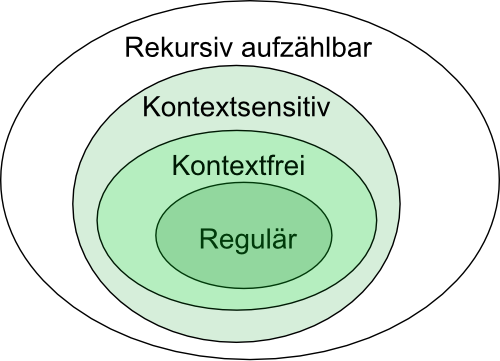
\includegraphics[width=0.7\textwidth]{Chomsky-Hierarchie.png}
				\caption{Chomsky-Hierarchie der formalen Sprachen}
				\label{fig:chomsky-hierarchie}
			\end{figure}
			
			
			\subsubsection*{1. Reguläre Grammatik (Typ-3-Grammatik)}
			
			\textbf{Eigenschaften:}
			\begin{itemize}
				\item Produktionsregeln haben die Form:  
				\( A \rightarrow aB \) oder \( A \rightarrow a \)  
				(\( A, B \) sind Nichtterminale, \( a \) ist ein Terminalsymbol)
				\item Es ist nur eine sehr eingeschränkte Form von Rekursion erlaubt.
				\item Sie erzeugt genau die \textbf{regulären Sprachen}.
			\end{itemize}
			
			\textbf{Beispiel:}
			\[
			S \rightarrow aS \mid bS \mid \epsilon
			\]
			Erzeugt alle Wörter über dem Alphabet \( \{a, b\} \): \( L = \{a, b\}^* \)
			
			\vspace{1em}
			
			\subsubsection*{2. Kontextfreie Grammatik (Typ-2-Grammatik)}
			
			\textbf{Eigenschaften:}
			\begin{itemize}
				\item Produktionsregeln haben die Form:  
				\( A \rightarrow \gamma \), wobei \( A \) ein Nichtterminal und \( \gamma \in (V \cup \Sigma)^* \) ist
				\item Das linke Seiten der Regel besteht aus genau \textbf{einem} Nichtterminal
				\item Es sind auch verschachtelte Strukturen und Rekursion möglich
				\item Sie erzeugt die \textbf{kontextfreien Sprachen}
			\end{itemize}
			
			\textbf{Beispiel:}
			\[
			S \rightarrow aSb \mid \epsilon
			\]
			Erzeugt die Sprache:  
			\[
			L = \{ a^n b^n \mid n \geq 0 \}
			\]
			
			\vspace{1em}
			
			\subsubsection*{Hauptunterschiede}
			
			\begin{itemize}
				\item Reguläre Grammatiken können nur sehr einfache Strukturen beschreiben (keine verschachtelten Abhängigkeiten).
				\item Kontextfreie Grammatiken erlauben rekursive, symmetrische Strukturen wie Klammerausdrücke oder geschachtelte Blöcke.
				\item Reguläre Sprachen sind eine Teilmenge der kontextfreien Sprachen:
				\[
				\text{regulär} \subset \text{kontextfrei}
				\]
			\end{itemize}
			
			\textbf{Fazit:}  
			Reguläre Grammatiken sind einfacher, aber auch eingeschränkter. Kontextfreie Grammatiken sind flexibler und können komplexere Strukturen modellieren.
			
			
			\item Was ist eine Grammatik, und aus welchen Komponenten besteht sie?\\
			
			In der formalen Sprachtheorie beschreibt eine \textbf{Grammatik} die Regeln, nach denen gültige Wörter (bzw. Sätze) einer formalen Sprache gebildet werden können.
			
			\subsubsection*{Definition einer Grammatik}
			
			Eine Grammatik ist ein Tupel:
			\[
			G = (V, \Sigma, P, S)
			\]
			
			\textbf{Dabei gilt:}
			\begin{itemize}
				\item \( V \): endliche Menge der \textbf{Nichtterminalsymbole} (Variablen), z.\,B. \( \{S, A, B\} \)
				\item \( \Sigma \): endliche Menge der \textbf{Terminalsymbole} (Alphabet), z.\,B. \( \{a, b\} \)  
				(\( V \cap \Sigma = \emptyset \))
				\item \( P \): endliche Menge von \textbf{Produktionsregeln} der Form \( \alpha \rightarrow \beta \), wobei \( \alpha, \beta \in (V \cup \Sigma)^* \) und \( \alpha \neq \epsilon \)
				\item \( S \in V \): \textbf{Startsymbol}, von dem die Ableitungen ausgehen
			\end{itemize}
			
			\subsubsection*{Beispiel einer einfachen Grammatik}
			
			\begin{itemize}
				\item Nichtterminale: \( V = \{S\} \)
				\item Terminale: \( \Sigma = \{a, b\} \)
				\item Produktionsregeln: \( P = \{S \rightarrow aSb,\ S \rightarrow \epsilon\} \)
				\item Startsymbol: \( S \)
			\end{itemize}
			
			\textbf{Diese Grammatik erzeugt die Sprache:}
			\[
			L = \{ a^n b^n \mid n \geq 0 \}
			\]
			→ also Wörter mit gleich vielen \( a \)- und \( b \)-Symbolen, wobei alle \( a \)'s vor den \( b \)'s stehen.
			
			\subsubsection*{Fazit}
			
			Eine formale Grammatik besteht aus vier Komponenten und definiert eine Sprache durch regelgeleitete Ableitungen. Sie ist ein zentrales Konzept in der formalen Sprachtheorie, Compilerbau und theoretischen Informatik.
			
			\item Erklären Sie den Unterschied zwischen Terminal- und Nichtterminalsymbolen.\\
			
			In einer formalen Grammatik unterscheidet man zwei Arten von Symbolen:
			
			\subsubsection*{1. Terminalsymbole (\( \Sigma \))}
			
			\begin{itemize}
				\item Die \textbf{Terminalsymbole} sind die Zeichen des Alphabets der Sprache.
				\item Sie sind die Endprodukte der Ableitung, aus denen die Wörter der Sprache bestehen.
				\item Terminalsymbole können nicht weiter ersetzt werden.
				\item Beispiel: \( \Sigma = \{a, b\} \) – die Buchstaben, die später in den erzeugten Wörtern vorkommen.
			\end{itemize}
			
			\subsubsection*{2. Nichtterminalsymbole (\( V \))}
			
			\begin{itemize}
				\item Die \textbf{Nichtterminalsymbole} dienen als Platzhalter oder Variablen im Ableitungsprozess.
				\item Sie werden im Laufe der Ableitung durch andere Nichtterminale oder Terminale ersetzt.
				\item Die Ableitung beginnt beim \textbf{Startsymbol}, das immer ein Nichtterminal ist.
				\item Beispiel: \( V = \{S, A, B\} \)
			\end{itemize}
			
			\subsubsection*{Gegenüberstellung}
			
			\begin{tabular}{|l|p{6cm}|p{6cm}|}
				\hline
				\textbf{Aspekt} & \textbf{Nichtterminalsymbole} & \textbf{Terminalsymbole} \\
				\hline
				Rolle & Platzhalter im Ableitungsprozess & Zeichen des endgültigen Wortes \\
				\hline
				Ableitung & Werden durch Regeln ersetzt & Bleiben unverändert \\
				\hline
				Beispiel & \( S \rightarrow aSb \) & \( a, b \) \\
				\hline
			\end{tabular}
			
			\vspace{1em}
			
			\textbf{Fazit:}  
			Nichtterminalsymbole steuern den Aufbau eines Wortes und werden im Ableitungsprozess ersetzt, während Terminalsymbole die tatsächlichen Buchstaben der Sprache darstellen und das endgültige Ergebnis bilden.
			
			\item Was bedeutet eine kontextfreie Grammatik (CFG)? Geben Sie ein Beispiel.\\
			
			Eine \textbf{kontextfreie Grammatik (engl. context-free grammar, CFG)} ist ein formales System zur Beschreibung von Sprachen, bei dem jede Produktionsregel nur ein einzelnes Nichtterminal auf der linken Seite hat.
			
			\subsubsection*{Formale Definition}
			
			Eine kontextfreie Grammatik ist ein Tupel:
			\[
			G = (V, \Sigma, P, S)
			\]
			mit:
			
			\begin{itemize}
				\item \( V \): Menge der \textbf{Nichtterminalsymbole}
				\item \( \Sigma \): Menge der \textbf{Terminalsymbole}, \( V \cap \Sigma = \emptyset \)
				\item \( P \): Menge der \textbf{Produktionsregeln} der Form \( A \rightarrow \gamma \), wobei \( A \in V \), \( \gamma \in (V \cup \Sigma)^* \)
				\item \( S \in V \): \textbf{Startsymbol}
			\end{itemize}
			
			\textbf{Merkmal:}  
			Jede Regel hat links genau ein Nichtterminalsymbol. Die Ersetzung ist unabhängig vom Kontext, in dem das Symbol steht – daher "kontextfrei“.
			
			\subsubsection*{Beispiel einer CFG}
			
			Gegeben sei folgende Grammatik:
			
			\begin{itemize}
				\item \( V = \{S\} \)
				\item \( \Sigma = \{a, b\} \)
				\item \( P = \{S \rightarrow aSb,\ S \rightarrow \epsilon\} \)
				\item \( S \): Startsymbol
			\end{itemize}
			
			\textbf{Erzeugte Sprache:}
			\[
			L = \{ a^n b^n \mid n \geq 0 \}
			\]
			
			\textbf{Beispielhafte Ableitungen:}
			\begin{align*}
				S &\Rightarrow \epsilon \\
				S &\Rightarrow aSb \Rightarrow ab \\
				S &\Rightarrow aSb \Rightarrow aaSbb \Rightarrow aabb \\
				S &\Rightarrow aSb \Rightarrow aaSbb \Rightarrow aaaSbbb \Rightarrow aaabbb
			\end{align*}
			
			\subsubsection*{Fazit}
			
			Eine kontextfreie Grammatik erlaubt die Beschreibung von strukturierten, verschachtelten Sprachen wie Klammerausdrücken, Programmiersprachen oder \( a^n b^n \). Sie ist mächtiger als eine reguläre Grammatik und spielt eine zentrale Rolle in der Informatik.
			
			\item Stellen Sie einen Vergleich zwischen Regulären und Kontextfreien Grammatik.\\
			\subsection*{Vergleich: Reguläre vs. Kontextfreie Grammatiken}
			
			\textbf{Reguläre Grammatiken (Typ-3)} und \textbf{Kontextfreie Grammatiken (Typ-2)} gehören beide zur Chomsky-Hierarchie, unterscheiden sich jedoch in Ausdrucksstärke und Struktur.
			
			\vspace{1em}
			
			\begin{tabularx}{\textwidth}{|l|X|X|}
				\hline
				\textbf{Kriterium} & \textbf{Reguläre Grammatik (Typ-3)} & \textbf{Kontextfreie Grammatik (Typ-2)} \\
				\hline
				Produktionsregeln & Nur in der Form \( A \rightarrow aB \) oder \( A \rightarrow a \) & In der Form \( A \rightarrow \gamma \), wobei \( \gamma \in (V \cup \Sigma)^* \) \\
				\hline
				Linke Seite der Regel & Ein Nichtterminalsymbol & Ein Nichtterminalsymbol \\
				\hline
				Rechte Seite der Regel & Maximal ein Terminal gefolgt von einem Nichtterminal oder nur ein Terminal & Beliebige Kombination aus Terminalen und Nichtterminalen \\
				\hline
				Ausdrucksstärke & Einfach, keine verschachtelten Strukturen & Unterstützt rekursive und verschachtelte Strukturen \\
				\hline
				Erkennbarkeit & Mit endlichen Automaten (DFA/NFA) & Mit Kellerautomaten (PDA) \\
				\hline
				Typische Anwendung & Reguläre Ausdrücke, einfache Mustererkennung & Programmiersprachen, mathematische Ausdrücke \\
				\hline
				Beispiel-Sprache & \( L = \{a^n \mid n \geq 0\} \) & \( L = \{a^n b^n \mid n \geq 0\} \) \\
				\hline
			\end{tabularx}
			
			\vspace{1em}
			
			\subsubsection*{Zusammenfassung}
			
			\begin{itemize}
				\item \textbf{Reguläre Grammatiken} sind einfach und effizient, aber in ihrer Ausdrucksstärke eingeschränkt.
				\item \textbf{Kontextfreie Grammatiken} sind flexibler und können auch komplexe, verschachtelte Strukturen modellieren.
				\item Jede reguläre Sprache ist auch kontextfrei, aber nicht jede kontextfreie Sprache ist regulär:
				\[
				\text{regulär} \subset \text{kontextfrei}
				\]
			\end{itemize}
			
			
			\item Sind Programmiersprachen wie beispielsweise Java oder C++ kontext-
			frei oder regulär.\\

			Programmiersprachen wie \textbf{Java}, \textbf{C++}, \textbf{Python} usw. sind \textbf{nicht regulär}, aber in weiten Teilen \textbf{kontextfrei}.
			
			\subsubsection*{Begründung:}
			
			\begin{itemize}
				\item Die Syntax von Programmiersprachen (z.\,B. Schleifen, Anweisungen, Funktionsdefinitionen) lässt sich meist durch eine \textbf{kontextfreie Grammatik (CFG)} beschreiben.
				\item Die lexikalische Struktur (z.\,B. Schlüsselwörter, Operatoren, Literale) kann hingegen durch \textbf{reguläre Ausdrücke} erkannt werden.
			\end{itemize}
			
			\subsubsection*{Kombiniertes Parsing-Verfahren}
			
			Typische Compiler nutzen zwei Phasen:
			
			\begin{itemize}
				\item \textbf{Scanner (Lexer):} erkennt Tokens mit Hilfe regulärer Ausdrücke (→ regulär)
				\item \textbf{Parser:} analysiert den Satzbau auf Basis einer kontextfreien Grammatik (→ kontextfrei)
			\end{itemize}
			
			\subsubsection*{Grenzen der Kontextfreiheit}
			
			Einige Sprachaspekte wie z.\,B.:
			\begin{itemize}
				\item Namensauflösung (Gültigkeit von Bezeichnern)
				\item Typkompatibilität
				\item Sichtbarkeitsbereiche (Scopes)
			\end{itemize}
			
			… lassen sich \textbf{nicht mit einer kontextfreien Grammatik beschreiben}, sondern erfordern eine \textbf{semantische Analyse} — also zusätzliche Regeln außerhalb der Grammatik.
			
			\subsubsection*{Fazit}
			
			\begin{quote}
				Die \textbf{Syntax moderner Programmiersprachen} ist im Allgemeinen \textbf{kontextfrei}, aber nicht vollständig durch eine kontextfreie Grammatik erfassbar. Ihre lexikalische Struktur ist regulär, ihre semantischen Aspekte erfordern zusätzliche Verarbeitung.
			\end{quote}
			
			\item Erstellen Sie eine kontextfreie Grammatik der Binärzahlen.
			
			Eine kontextfreie Grammatik \( G \) erzeugt Binärzahlen:
			\begin{itemize}
				\item Terminale: \( \{0, 1\} \)
				\item Nichtterminale: \( \{S\} \)
				\item Startsymbol: \( S \)
				\item Produktionsregeln:
				\begin{align*}
					S &\to 0S \mid 1S \mid 0 \mid 1
				\end{align*}
			\end{itemize}
			
			\section*{Vergleichsaufgabe: Reguläre vs. Kontextfreie Grammatik}
			
			\textbf{Aufgabenstellung:}  
			Gegeben sind zwei Grammatiken \( G_1 \) und \( G_2 \). Bestimmen Sie für beide:
			\begin{enumerate}
				\item Die Sprache \( L(G) \), die sie erzeugen.
				\item Ob die Grammatik regulär oder kontextfrei ist.
				\item Begründen Sie Ihre Entscheidung anhand der Regeln.
			\end{enumerate}
			
			\vspace{1em}
			
			\subsection*{Grammatik \( G_1 \)}
			
			\begin{itemize}
				\item \( V = \{S\} \)
				\item \( \Sigma = \{a, b\} \)
				\item \( P = \{S \rightarrow aS \mid bS \mid \epsilon\} \)
				\item Startsymbol: \( S \)
			\end{itemize}
			
			\subsubsection*{Lösung zu \( G_1 \)}
			
			\begin{itemize}
				\item Diese Grammatik erzeugt alle Wörter über \( \{a, b\} \), also:
				\[
				L(G_1) = \{a, b\}^*
				\]
				\item Alle Regeln haben die Form: \( S \rightarrow aS \), \( S \rightarrow bS \), \( S \rightarrow \epsilon \)
				\item Das entspricht genau einer \textbf{rechtslinearen regulären Grammatik}.
				\item \textbf{Fazit:} \( G_1 \) ist \textbf{regulär}.
			\end{itemize}
			
			\vspace{1em}
			
			\subsection*{Grammatik \( G_2 \)}
			
			\begin{itemize}
				\item \( V = \{S\} \)
				\item \( \Sigma = \{a, b\} \)
				\item \( P = \{S \rightarrow aSb \mid \epsilon\} \)
				\item Startsymbol: \( S \)
			\end{itemize}
			
			\subsubsection*{Lösung zu \( G_2 \)}
			
			\begin{itemize}
				\item Die Regel \( S \rightarrow aSb \) erlaubt es, ein \texttt{a} am Anfang und ein \texttt{b} am Ende hinzuzufügen.
				\item Damit entsteht z.\,B.:
				\[
				\epsilon,\ ab,\ aabb,\ aaabbb,\dotsc
				\]
				\item Die Sprache ist:
				\[
				L(G_2) = \{ a^n b^n \mid n \geq 0 \}
				\]
				\item Diese Sprache ist \textbf{nicht regulär} (Pumping-Lemma!), aber sie ist \textbf{kontextfrei}.
				\item Die Regel \( S \rightarrow aSb \) ist \textbf{nicht rechtslinear}, da das Nichtterminal \( S \) in der Mitte steht.
				\item \textbf{Fazit:} \( G_2 \) ist \textbf{kontextfrei}, aber nicht regulär.
			\end{itemize}
			
			\vspace{1em}
			
			\subsection*{Zusammenfassung:}
			
			\begin{tabular}{|c|l|l|}
				\hline
				\textbf{Grammatik} & \textbf{Sprache} & \textbf{Typ} \\
				\hline
				\( G_1 \) & \( \{a, b\}^* \) & Regulär \\
				\hline
				\( G_2 \) & \( \{a^n b^n \mid n \geq 0\} \) & Kontextfrei, nicht regulär \\
				\hline
			\end{tabular}
			
			\vspace{1em}
			
			\textbf{Erkenntnis:}  
			Reguläre Grammatiken können nur lineare Strukturen erzeugen.  
			Kontextfreie Grammatiken sind mächtiger und können auch verschachtelte Strukturen wie \( a^n b^n \) erzeugen.
			
			
			
		\end{enumerate}	
		

	
\end{document}
